\clearpage
\section{Software architecture and implementation walkthrough}
\label{sec:software}

\subsection{A component map for readers of the repository}
The research system and classroom interface share environment and policy
components, but have different responsibilities. Training may update parameters;
the demo may only load and evaluate them. The distinction prevents a successful
UI interaction from being mistaken for an online learning result.

\begin{table}[htbp]\centering\small
\begin{tabularx}{\textwidth}{lY}\toprule
Repository component & Responsibility and contract\\\midrule
\texttt{src/models} & Vector Q-network, per-head targets, PPO actor/critic, PopArt and Lunar GAE.\\
\texttt{src/core} & Replay, episode preferences, Pareto archive and credit-assignment utilities.\\
\texttt{src/curriculum} & Scores over a fixed preference pool and uniform-floor sampling.\\
\texttt{src/envs} & Environment creation, reward wrappers, declared shifts and replay support.\\
\texttt{src/evaluation} & Protocol loading, rollout records, metrics and fail-closed qualification.\\
\texttt{src/demo} & Frozen-policy adapter, two-panel state machine and local HTTP API.\\
\texttt{demo/interactive} & English HTML/CSS/JavaScript interface and cosmetic Canvas renderer.\\
\texttt{research/} & Versioned claims, experiments, literature, raw-result evidence and sessions.\\
\texttt{scripts/} & Explicit training, audit, packaging, report and verification entry points.\\\bottomrule
\end{tabularx}
\caption{Source responsibilities. Generated checkpoints and runtime environments are not Git source files.}
\end{table}

\begin{figure}[htbp]\centering
\resizebox{\textwidth}{!}{\begin{tikzpicture}[node distance=12mm and 10mm]
\node[block] (ui) {English browser UI\\sliders / pause / step};
\node[block,right=of ui] (api) {Local HTTP API\\generation + tick ID};
\node[block,right=of api] (runtime) {Two-panel runtime\\isolated episode states};
\node[block,below=of runtime] (model) {Frozen PPO actor\\SHA-256 checked};
\node[block,left=of model] (physics) {Actual environment\\vector rewards / flags};
\node[block,left=of physics] (view) {Snapshot + trace\\styled or native view};
\draw[flow] (ui)--(api);\draw[flow] (api)--(runtime);
\draw[flow] (runtime)--(model);\draw[flow] (model)--(physics);
\draw[flow] (physics)--(view);\draw[flow] (view)--(ui);
\node[below=10mm of physics,font=\sffamily\small,text=Muted,align=center]
{No gradient updates or checkpoint selection.\\Presentation diagnostics remain separate from research evidence.};
\end{tikzpicture}
}
\caption{Inference boundary. The browser requests transitions from a local
server; it does not invent rewards or move the environment independently.
Training sources and evaluation evidence remain separate from UI state.}
\end{figure}

\subsection{One action through the implemented stack}
An environment reset constructs the declared nominal configuration, initializes
the episode seed and obtains its first observation. The runtime validates the
preference as a finite simplex vector. For a PPO actor, objective-wise state
features are merged according to that preference; categorical action
probabilities are computed, and the demonstration selects their argmax.
The action enters the actual environment, which returns a vector reward,
next observation and separate termination/truncation flags. The runtime adds
raw components and discounted, fixed-scale components to separate counters.
Only then does the browser receive the next state and draw it.

The policy loader first compares the checkpoint bytes with the recorded
SHA-256 digest and loads the exported weights with the restricted weights-only
loader. Models are put in evaluation mode and gradients disabled. A changed
checkpoint fails loading. Localization changes labels and explanatory text;
it does not alter seeds, network parameters, action ordering, reward scales,
discounting or physics. The English package retains the original checkpoint
hashes in its own configuration and records the base-configuration hash.

\subsection{Two-panel state and fault handling}
Both panels start from matched seeds and the same model. Each keeps its own
observation, return vector, end flags and trajectory. Isolated random state
prevents one panel's Minecart sampling from consuming the other's randomness.
The reference preference is fixed at its declared default. The user preference
is pending until reset, unless the live option is explicitly enabled.

Requests carry a generation and monotonically increasing tick ID. A duplicate
tick with the same payload returns its prior result; a conflicting duplicate or
stale generation is rejected. Failed transition calls halt the session rather
than automatically executing another step. A reset/reload is required after
an engine fault. Server binding is local-only, and mutation requests require
the session token and a trusted local origin. These engineering protections
are not a substitute for exposing the app only on the local machine.

\clearpage
\section{English demonstration and visual evidence}
\label{sec:visual-demo}
The following screenshots were captured from the English application in a real
headless Microsoft Edge browser. They use the existing pilot/confirmation
checkpoint exports, unchanged. Each capture follows a fixed presentation horizon
(up to 80 steps for Lunar and 120 for Minecart, stopping at episode completion).
The screenshots are interface and inference witnesses, not selected successful
episodes, independent replications, or evidence for a new learning claim.

\begin{figure}[H]\centering
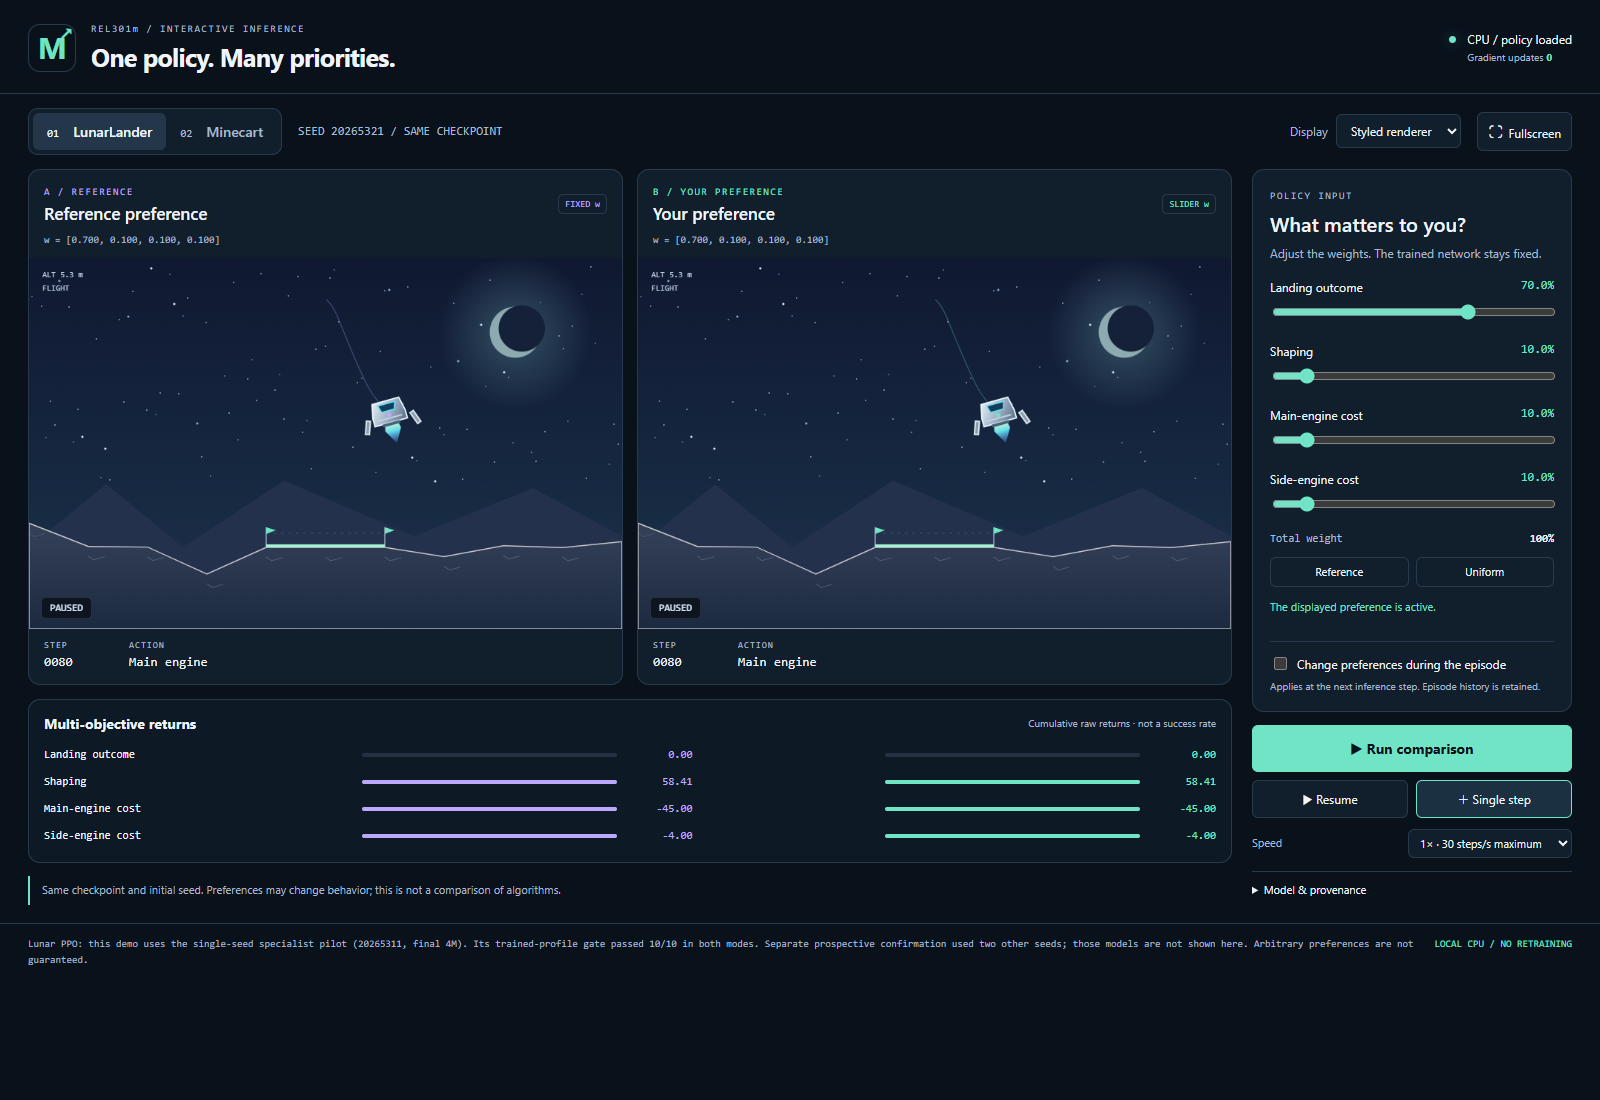
\includegraphics[width=\textwidth]{Figures/english-demo/lunar-english.png}
\caption{English LunarLander interface with actual policy inference. The two
panels share pilot checkpoint 20265311 and the initial seed. Objective weights,
action names, raw returns and provenance are visible; styled graphics use
environment coordinates. A frame in flight does not certify a completed landing.}
\end{figure}

\begin{figure}[H]\centering
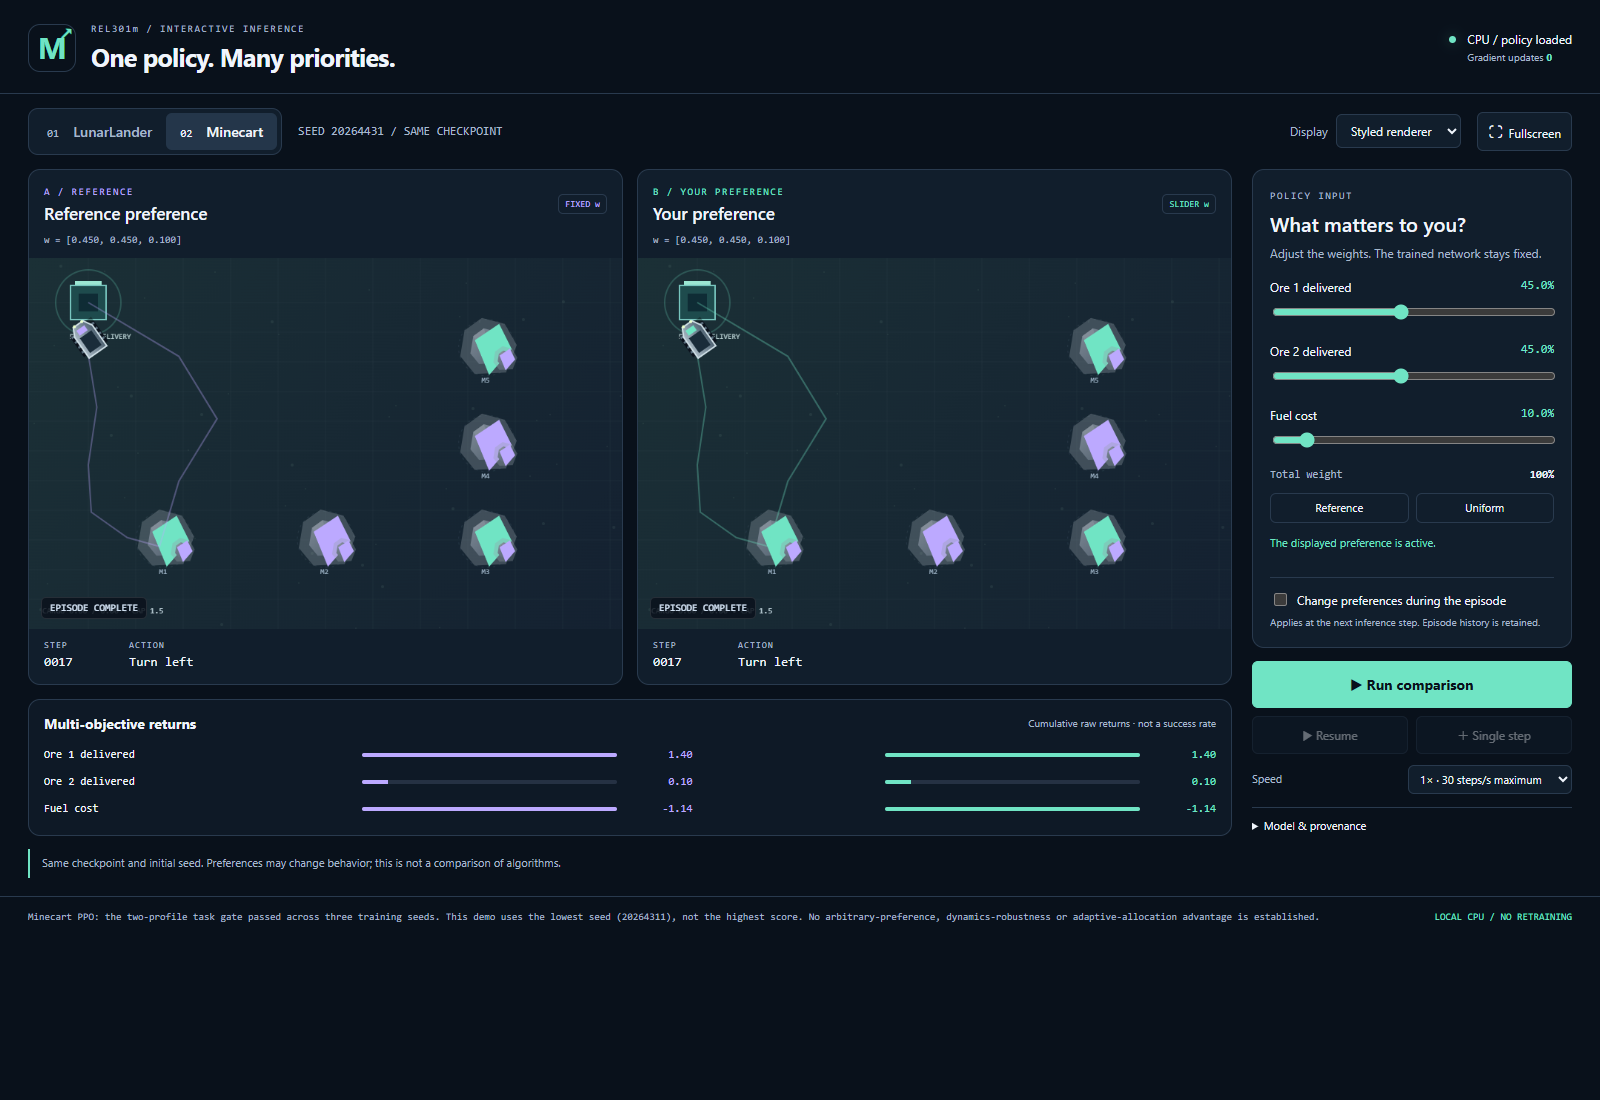
\includegraphics[width=\textwidth]{Figures/english-demo/mine-english.png}
\caption{English Minecart interface. The displayed actor is confirmation seed
20264311, selected by the lowest-seed rule. Ore and fuel components are distinct;
an attractive renderer does not change the underlying policy or imply that all
preferences are effective.}
\end{figure}

\begin{figure}[H]\centering
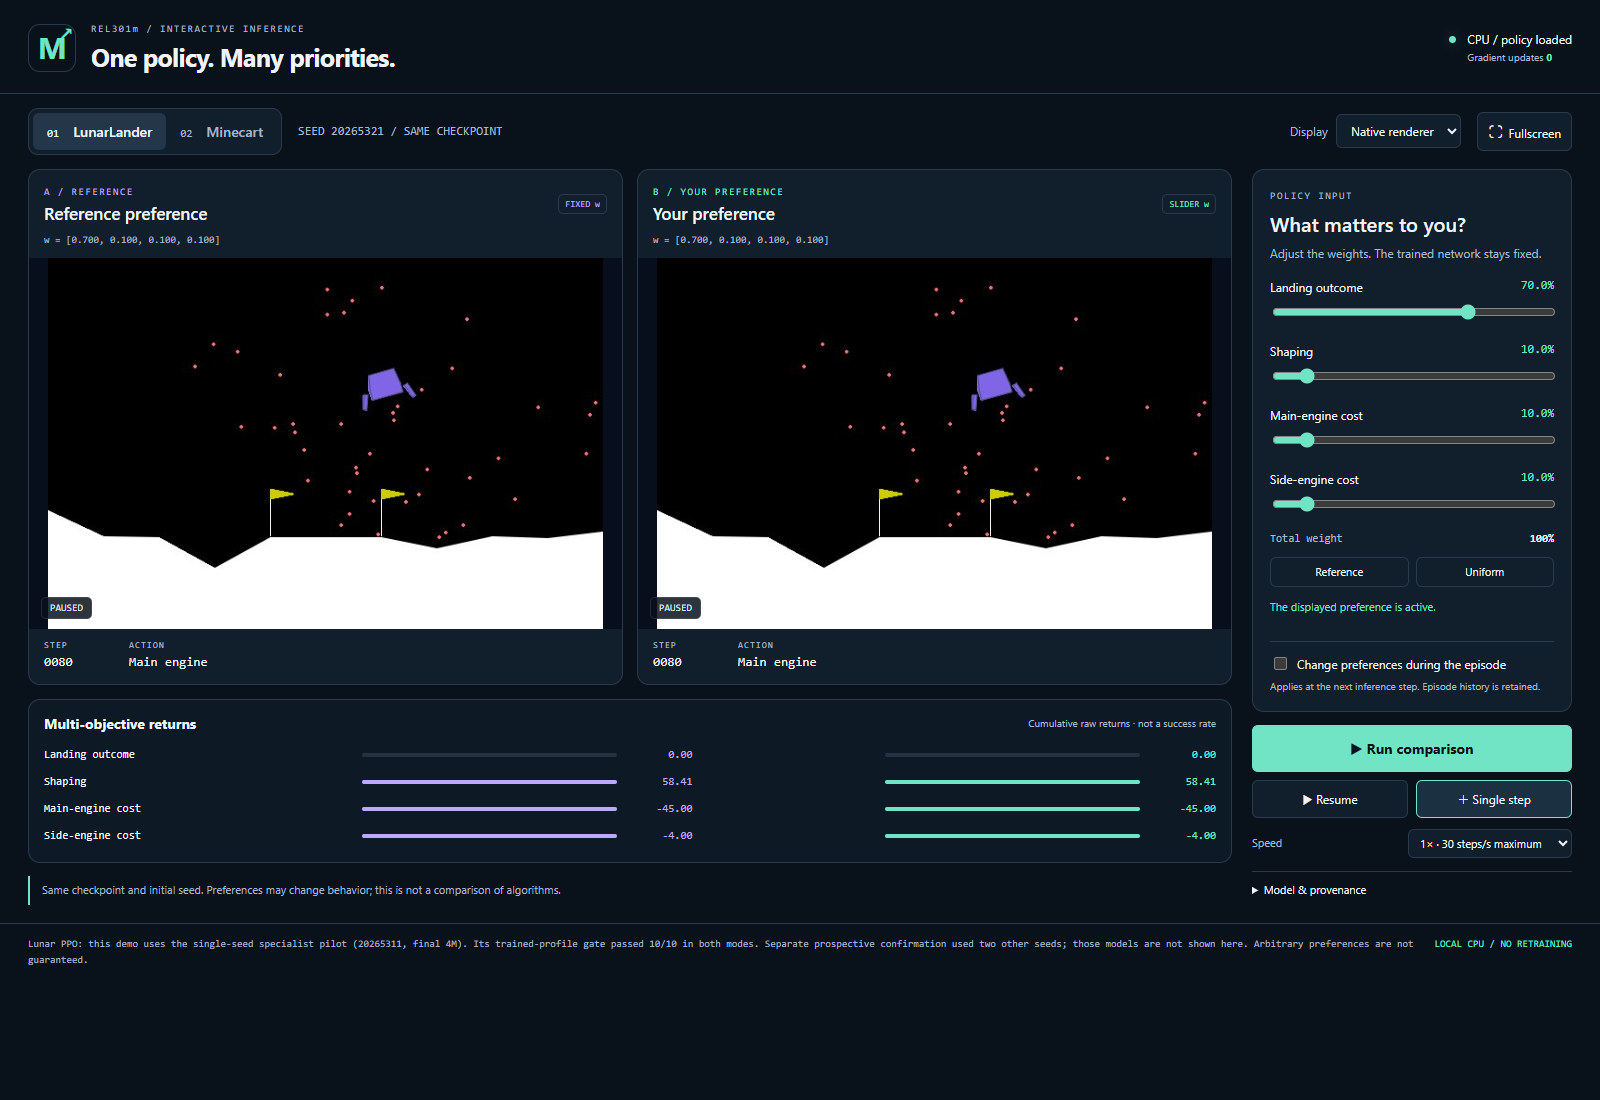
\includegraphics[width=.94\textwidth]{Figures/english-demo/lunar-native.png}
\caption{Original Lunar renderer at the same saved presentation state as its
styled screenshot. Switching display mode executes no physics transitions.
Native frames permit a direct check against the decorative Canvas view.}
\end{figure}

\subsection{A reproducible classroom walkthrough}
\begin{enumerate}
\item Start the English package with Python 3.11 and open its localhost URL.
The interface starts paused; use \textbf{Single step} to inspect an action.
\item Explain the four Lunar objectives and the three Minecart objectives.
Costs are negative reward components. Increasing their weight expresses greater
importance on avoiding that cost; it does not add fuel to the simulator.
\item Move a slider and show the pending-preference message. In ordinary mode,
no transition or model update occurs until \textbf{Run comparison} resets the
two panels. Weight redistribution preserves a total of 100\%.
\item Compare the declared default with a uniform or ore-heavy preference.
Report the observed behavior without promising that every weight has been learned.
The same model can select the same action at different preferences.
\item Enable live preference changes, take a step and explain the history
warning. Different histories prevent a causal comparison from that point alone.
Reset before drawing a matched-initial-state comparison.
\item Switch to the native renderer and export a trace. Use the report's
evidence tables for task conclusions, rather than the appearance of one run.
\end{enumerate}

\subsection{What the displayed numbers mean}
For episode length $T$, the app retains
\[
G^{\mathrm{raw}}_j=\sum_{t=0}^{T-1}r_{t,j},\qquad
G^{\mathrm{scaled}}_j=\sum_{t=0}^{T-1}\gamma^t c_jr_{t,j},\qquad
U_w=w^\top G^{\mathrm{scaled}},
\]
where $c_j$ is the frozen protocol scale. The UI return bars show raw components,
whose units and magnitudes differ. Their relative bar lengths are a visual
comparison between the panels for the same objective, not a cross-objective
normalization or percentage of task completion. A positive landing component
alone is also weaker than the audit's native pad-position gate.

\section{Reproduction, verification and hand-in checklist}
\subsection{Reconstructing the right runtime}
Research targets Python 3.11 with direct pins in \texttt{requirements.txt}.
Use a dedicated environment; do not reuse Python installations or compiled
packages across Windows and Linux. The current checkout is hosted in WSL
Ubuntu-24.04. Its inspected Linux system/baseline environments supplied Python
3.12, so a clean full Linux reconstruction is not certified by this edition.
The existing standalone Windows demo environment uses Python 3.11.18.
QA dependencies are isolated outside the repository, and their location is
recorded in the session verification note.

Source code and compact result records are in Git. Checkpoints, installed
runtimes, caches and generated packages are local ignored artifacts. A clone
can inspect code and evidence but needs a separately supplied pretrained
package to run these specific actors. The root Windows launcher historically
expects a relative virtual environment and a prepared package; it is not a
fresh-clone installer. The explicit English package entry point avoids guessing
which historical package is active.

\begin{verbatim}
# From an English package with Python 3.11 dependencies installed:
python launch.py --port 8765
# Open http://127.0.0.1:8765; Ctrl+C stops the local server.
\end{verbatim}

\subsection{Verification scope}
Backend tests cover preference validation, preserved terminal semantics,
duplicate requests, source hashes and rendering state. Frontend tests cover
pending/live weights, pause/step, reset, errors and simplex redistribution.
Real-browser checks exercise both actual environments, English visible text,
native rendering without extra steps, mobile layout and traceable screenshots.
These layers complement each other: a fake DOM test is not browser rendering,
and a browser screenshot is not proof of policy competence.

The report's deterministic auditor resolves its LaTeX inputs, checks citation
keys against the versioned library, resolves graphics and evidence paths and
checks bounded result counts/utilities against recorded data. It does not
independently recertify every full-text literature reading or infer causality
from the negative-to-positive research chronology. Visual page inspection is
required in addition to compilation and text extraction.

\begin{verbatim}
python scripts/research_harness.py doctor
python -m ruff format --check .
python -m ruff check .
python -m mypy src scripts
python -m pytest -q
python -m bandit -q -r src scripts -ll
python -m compileall -q src scripts tests
git diff --check
\end{verbatim}

The current working tree contains preexisting, uncommitted presentation work.
Whole-tree lint can include those files; a submission receipt must distinguish
them from the tracked Python files in the reviewed change. Unix-only ARIS tests
and missing historical-checkpoint integrations must be reported as skips, not
passes. No test command here authorizes renewed research training or final-test access.

\subsection{Deliverables and known exclusions}
This edition supplies the English PDF with editable LaTeX source, existing
bibliography, data-derived charts, deterministic architecture figures and real
English demo screenshots. The demo retains its fixed trained models. Earlier
packages and evidence remain preserved. No video is required: that term in the
request was clarified as a dictation error. Additional slides, fresh training,
best-seed promotion, public hosting and final-test evaluation are outside this
edition. Lecturer acceptance and any department-specific rubric remain external.
